% INTRODUCTION
%

%
%\part{Introduction}
\chapter{Introduction}
\label{chap:intro}

%\cleanchapterquote{You can’t do better design with a computer, but you can speed up your work enormously.}{Wim Crouwel}{(Graphic designer and typographer)}

%In the field of second-language education, pronunciation has traditionally been given less attention than other areas such as grammar or vocabulary \citep{Derwing2005}. One reason for this may be that pronunciation is best taught through one-on-one instruction, which is not often possible in the traditional classroom setting. Hence the attraction of Computer-Assisted Pronunciation Training (CAPT) systems, which have the potential to automatically provide highly individualized analysis of learner errors, and feedback on how to correct them and achieve more intelligible 
%and native-like 
%pronunciation in the target language \citep{Witt2012}. 

%Something about how there's not much CAPT for German?

For students with French as their first language (L1) who are learning German as a second language (L2), the sound system of the L2 can pose a variety of difficulties, one of the most important and interesting of which is the way in which certain syllables in German words are accentuated more than others, a phenomenon referred to as lexical stress. Learning to navigate German lexical stress is especially challenging for L1 French speakers, because this phenomenon is realized very differently in the French language. 

Computer-Assisted Pronunciation Training (CAPT) systems
%, which 
have the potential to automatically provide highly individualized analysis of such learner errors, as well as feedback on how to correct them, and thus to help learners achieve more intelligible 
%and native-like 
pronunciation in the target language \citep{Witt2012}. 
%
The thesis project described here aims to advance 
%the state of the art of 
German CAPT %TODO too intense? reword
by creating a tool which will diagnose and offer feedback on lexical stress errors in the L2 German speech of L1 French speakers, in the hopes of ultimately helping these learners 
%become more sensitive to the lexical stress patterns of German and develop the ability to accurately realize these patterns in their speech. 
become more intelligible when speaking German.

%TODO move Context to after Objectives?
\section{Context: The IFCASL project}
\label{sec:intro:ifcasl}

This work has been conducted in the context of the ongoing research project ``Individualized Feedback in Computer-Assisted Spoken Language Learning (IFCASL)'' at Saarland University (Saarbrücken, Germany) and LORIA (Nancy, France). \TODO{more project info (ANR/DFG project no.? citation?)}
%TODO can I cite project proposal?

The goal of the IFCASL project is to take initial steps toward the development of a CAPT system targeting
%, on the one hand, 
native (L1) French speakers learning German as a foreign language (L2), 
as well as
%and on the other, 
L1 German speakers learning French as their L2. To this end, a bidirectional learner speech corpus has been recorded, comprising phonetically diverse utterances in French and German spoken by both native speakers and non-native speakers with the other language as L1 \citep{Fauth2014,Trouvain2013}.  While the project as a whole is thus also concerned with L1 German speakers learning French as L2, this thesis focuses exclusively on French L1 speakers learning German as L2. 

\TODO{Details about corpus (summary of corpus articles)}

\TODO{Remove the following paragraph?}
The German-language subset of the IFCASL corpus has been instrumental in training and testing the automatic diagnosis and feedback systems developed in this work. Furthermore, those systems have been designed with a view to contributing to the overall set of software developed in the context of the IFCASL project, such that they have been as compatible as possible with the other tools developed and used by the IFCASL team. %TODO reword that


\section{Objectives}
\label{sec:intro:objectives}

%		\begin{floatingfigure}[r]{.5\textwidth}
%			\centering
%			\vspace{-2em}
%			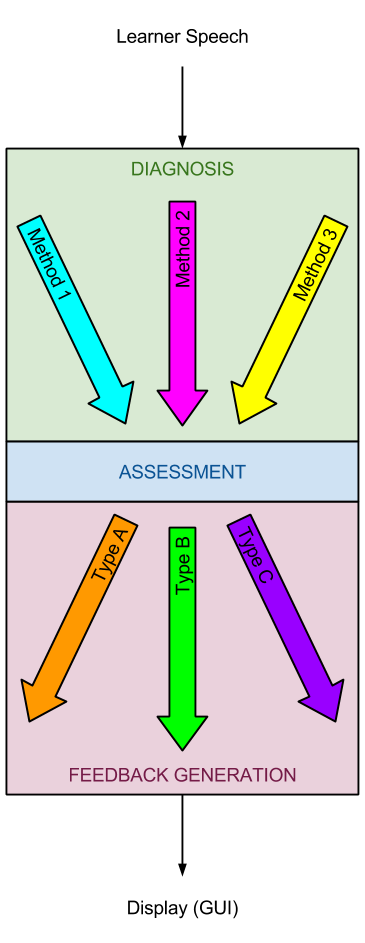
\includegraphics[width=.35\textwidth]{../img/hourglass}
%			\vspace{1em}
%			\caption{Conceptual diagram of the prototype CAPT tool.}
%			\label{fig:hourglass}
%			%\vspace{1em}
%		\end{floatingfigure}

The main objective of this work is to investigate the automatic treatment of lexical stress errors in the context of a CAPT system for French learners of German. This includes, on the one hand, an examination of the ways in which lexical stress errors of the type made by French L1 speakers when speaking German as L2 can be reliably detected and measured %TODO reword
automatically, and on the other, an exploration of the types of multimodal feedback on such errors that can be automatically delivered based on the aforementioned error detection. 
%
	\begin{figure}[thb] 
		\centering
		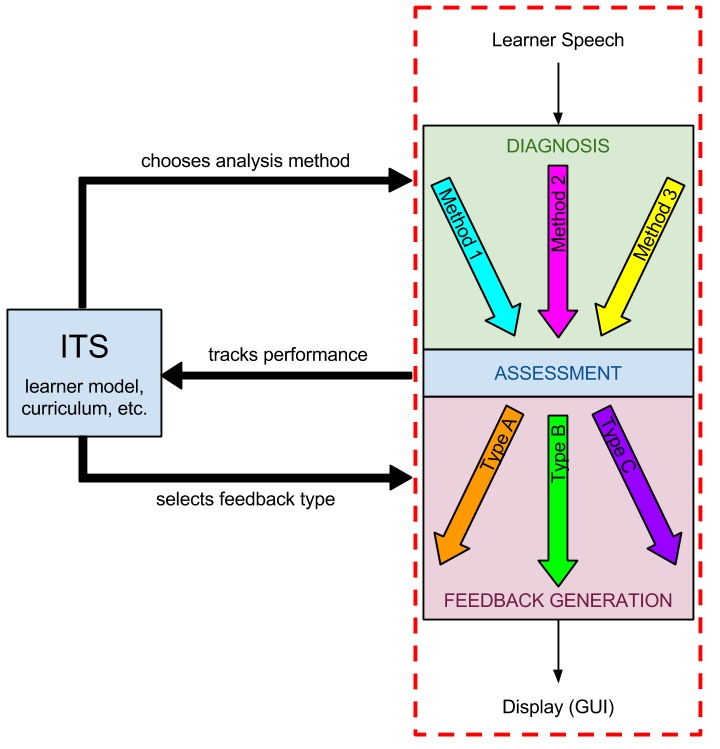
\includegraphics[height=.45\textheight]{../img/hourglass-ITS} 
		\caption[Conceptual diagram of the prototype lexical stress CAPT tool]{Conceptual diagram of the prototype lexical stress CAPT tool (demarcated by dotted line) and its possible function in the context of a more comprehensive Intelligent Tutoring System.}
		\label{fig:hourglass-ITS}
	\end{figure}
%
The outcome of these investigations is a prototype CAPT tool, illustrated in \cref{fig:hourglass-ITS},
which can diagnose lexical stress errors in different ways and present learners with different types of feedback on these errors.

This prototype tool has been developed with both instructional and research applications in mind.
Unlike with some existing tools for diagnosis pf and feedback on pronunciation errors, learners can interact with the tool and interpret its feedback independently, i.e. without the assistance of a human instructor at their side.
At the same time, researchers can use this modular system to study the impact of various assessment and feedback types on learner outcomes, user engagement, and other factors impacting the success of a CAPT system. 
%
Once more is known about which diagnosis/feedback types should be delivered to which learners in which situations, this tool could become a useful component to a fully-fledged CAPT system, in which learner models and other intelligent components automatically decide which modules of the tool to activate. 



\section{Thesis overview}
\label{sec:intro:overview}

\TODO{Add chapter names?}

\myemph{\Cref{chap:background}} introduces Computer-Assisted Pronunciation Training (CAPT) in the contexts of pronunciation teaching in foreign-language education and computer-based and intelligent tutoring systems, describing some relevant past work on CAPT systems. This chapter also briefly 
%outlines the differences in the lexical stress systems of French and German as well as 
introduces the phenomenon of lexical stress as it pertains to L1 French learners of German as L2, and outlines
the motivation for focusing on lexical stress errors in this work.

%TODO flesh out

\myemph{\Cref{chap:lexstress}} 
%explores lexical stress in the speech systems of French and German in more detail, describing relevant findings from past work on lexical stress and its acoustic correlates in these languages. 
%This chapter also 
describes original work on the annotation and analysis of lexical stress errors in the IFCASL sub-corpus of nonnative German speech produced by native French speakers.

\myemph{\Cref{chap:diagnosis}} details how the prototype CAPT tool diagnoses lexical stress errors in learner speech. It describes the methods used to automatically segment the learner's utterance, analyze the prosody of this utterance in terms of the relative pitch, duration, and intensity of the relevant syllables, and compare this analysis to one or more models of native pronunciation to produce a diagnosis.

\myemph{\Cref{chap:feedback}} describes the multimodal feedback options that the system can deliver, and how these feedback types are generated based on the analysis of the learner's speech described in the previous chapter. 

\myemph{\Cref{chap:system}} briefly introduces the tools that have been developed, and the technology used to build them. \TODO{skip this chapter?}

\myemph{\Cref{chap:conclusion}} summarizes the contributions of this work and outlines some 
possible directions for future work.
%interesting future directions to build on these contributions. %TODO rephrase that



%\section{Proposal overview}
%The remainder of this proposal is structured as follows.
%
%TODO update - this is the old overview from the proposal
%\Cref{chap:background} places this thesis in the context of existing research on CAPT, and motivates its specific focus on lexical stress errors.
%\Cref{chap:diagnosis} outlines the techniques to be explored for diagnosing lexical stress errors in learners' speech via automatic processing of acoustic correlates of these errors in a spoken utterance.
%\Cref{chap:feedback} describes the multimodal feedback types the system will aim to deliver, 
%%and how these could be generated automatically from 
%based on
%the analysis described in the previous section.
%\Cref{sec:conclusion} summarizes the proposal and the aims of the thesis.

